% File              : manual.tex
% Author            : Marcos Horro <marcos.horro@udc.gal>
% Date              : Mar 24 Dec 2019 19:31:10 MST
% Last Modified Date: Mér 25 Dec 2019 18:35:55 MST
% Last Modified By  : Marcos Horro <marcos.horro@udc.gal>
\documentclass[a4paper,12pt]{memoir}
% For TeXstudio users:
% !TeX spellcheck = en_US

\usepackage[ruled,vlined]{algorithm2e}
\usepackage{graphicx}
\usepackage{amsthm}
\usepackage{tikz}
\usetikzlibrary{arrows}

%\theoremstyle{definition}
\newtheorem{definition}{Definition}[]
\newtheorem{corollary}{Corollary}[]




% Title Page
\title{\textbf{MACVETH}: \textbf{M}ulti-dimensional \textbf{A}rray
    \textbf{C}-compiler for \textbf{VE}ctorizing
    \textbf{T}ensors for \textbf{H}PC applications}
\author{Marcos Horro}
\date{}

%%%%%%%%%%%%%%%%%%%%%%%%%%%%%%%%%%%%%
\begin{document}

\maketitle

%%%%%%%%%%%%%%%%%%%%%%%%%%%%%%%%%%%%%
\begin{abstract}
	This document presents the Multi-dimensional Array C-compiler for VEctorization
	and Transformation in HPC applications (MACVETH) compiler tool. Details
	regarding implementation and design decision are explained in detail. For
	specific implementation details refer to the proper source code, which is also
	documented using Doxygen.
\end{abstract}

\chapter{MACVETH}

Despite of the extraordinary performance with regard to the optimizations that
compilers (e.g. ICC, LLVM, gcc) may be able to do all over programs, they also
show limitations when it comes to vectorization. There are cases where either
they may not vectorize the code at all or even deliver worse performance than a
sequential version of it. This is a common scenario when the region of interest
in the code to vectorize is not regular. We may define the regularity of a code
as the presence of patterns whose accesses to the elements (e.g.
multi-dimensional arrays) are performed in a sequential and contiguous manner,
e.g. map operations. On the other hand, reductions are a type of operations
that, by nature,
do not fully exploit the capacity of vector operands. Current data placement or
packing techniques are meant just for loading and storing data from or to
memory, without performing any other logic than that. Potential improvements
regarding the vector occupancy by complex and smart packing techniques may lead
to major gains in performance. Picture the following example: within the same
loop we have two different and contiguous reductions. This is a common pattern
that can be found after the fusion of different loops, for instance, in codes
that perform convolutions. Assuming a vector size of four elements, a smart way
of computing this code is by

% Different ISA
In an orthogonal dimension, the quality of SIMD code is affected by the knowledge of the architecture where it is being compiled. Nevertheless, some information regarding the SIMD instructions performance may be missing or non-disclosed by the manufacturer. This information can be used to determine whether a vector operation is detrimental or not, i.e. for building a cost model. There may be architectures using the same ISA and, therefore, where the vectorization can be done using exactly the same instructions, but because of their architectural designs the performance may be different, leading to different approaches on each case. Thus, the only manner of disclosing this information is by reverse-engineering each architecture. This process is tedious and complex since there are many different instructions whose performance may be also vary depending on the packing of the data they use.


MACVETH is a source-to-source compiler which targets the vectorization of C/C++
codes. Thus, the input of this compiler is a non vectorized C/C++ code and the
output will be a SIMD-fashion C/C++ code (see Figure~\ref{fig:MACVETHarch}).
The name of the compiler stands for Multi-dimensional Array C-compiler for
VEctorizating Tensors for HPC applications. Besides, Macbeth, tragedy
written by William Shakespeare, represents the detrimental effects of human's
narcissism and vanity when looking for the power for its own benefits. As
opposed, MACVETH is composed by a set different layers and intermediate
representations that seek for the common purpose of improving performance. Last
but not least, the first and last letter of the acronym stand for the name of
the main author (Marcos Horro).

\begin{figure}
	\centering
	\includegraphics[width=\textwidth]{img/MACVETH.pdf}
	\caption{High-level picture of the MACVETH pipeline compiler.}
	\label{fig:MACVETHarch}
\end{figure}

\chapter{Intermediate Representations (IR)}



This compiler handles different abstraction levels or intermediate
representations for each step. As MACVETH is based in Clang~\cite{bib:clang},
the first abstraction layer lays on the Clang AST. This representation allows to
identify the regions of interest for the translation.

\section{MACVETH Expressions: MVExpr}
Clang implements complex expressions in order to handle any form or type of
code. They
provide many possibilities
when it comes to parse exactly the code. Nonetheless, in our case we are
interested in a small set of operations, so we created basically a wrap for this
purpose. MVExpr is an abstract class that can be specialized for any type we
want to represent from the Clang AST. Besides, the idea of this class is to
provide a set of non-standard transformations for the expressions, e.g.
unrolling. Thus, MVExpr are instantiated using a factory.

We have implemented the following specializations, which are enough in order to
represent any value reference:

\begin{itemize}
	\item \textbf{MVExprArray}: represents any N-dimensional expression in the
	      code. It
	      holds information of the number of dimensions and name or value of the
	      indices. This class is very useful when performing unrolling, as it 
	      provides methods for computing deltas between two indices of the same 
	      or different form, e.g. $(i+1)*2$ vs. $(i+1)*4$.
	\item \textbf{MVExprVar}: regardless the type of the variable, this
	      abstraction
	      represents, basically, any \texttt{DeclRefExpr} from the Clang AST.
	\item \textbf{MVExprLiteral}: any integer, float, double, char, etc. value.
	\item \textbf{MVExprFunc}: this is a recursive abstraction which holds the
	      name of the function and the parameters it receives. Parameters are also
	      MVExpr
	      type.
\end{itemize}

\section{Three-Address Code IR: TAC}
The Three-Address Code (TAC) representation used translates any statement ($S$)
into a
set of Single Stament Assignment (SSA) using quadruples, as described in
Definition~\ref{def:TAC}.

\theoremstyle{definition}
\begin{definition}\label{def:TAC}
	A three-address code is a 4-tuple TAC=(a,b,c,$\oplus$) which represents the
	assignment of the $b \oplus c$ operation as $a
		=
		b \oplus c$. If the $\oplus$ operator is unary then $c$ is null.
\end{definition}

In order to perform this translation, we have implemented the recursive process
is listed in
Algorithm~\ref{alg:stmtToTAC}. Each statement may be composed by a
concatenation of operations, which are split onto TACs respecting the
operational order. Therefore, we can conclude that any statement
can be represented as a set of TACs (formally stated in
Corollary~\ref{cor:TAC}).

\begin{algorithm}[H]\label{alg:stmtToTAC}
	\SetAlgoLined
	\KwIn{Stmt S}
	\KwResult{Set of TAC}
	L $\leftarrow$ \{\}\;
	Res $\leftarrow$ getResultOrTempReg(S)\;
	Lhs $\leftarrow$ getLHS(S)\;
	Rhs $\leftarrow$ getRHS(S)\;
	\If{isNonTerminal(Lhs)}{
		TAC $\leftarrow$ translateStmtToTAC(Lhs)\;
		addTacToList(L, TAC)\;
		Lhs $\leftarrow$ TAC.Res\;
	}
	\If{isNonTerminal(Rhs)}{
		TAC $\leftarrow$ translateStmtToTAC(Rhs)\;
		addTacToList(L, TAC)\;
		Rhs $\leftarrow$ TAC.Res\;
	}
	addTacToList(L, \{Res, Lhs, Rhs, getOp(S)\})\;
	return L\;
	\caption{translateStmtToTAC}
\end{algorithm}

\begin{corollary}\label{cor:TAC}
	Any statement $S$ can be represented as a set of interconnected TACs:
	$S = \{TAC\}$
\end{corollary}

This representation is widely used in compilers. The main advantages of it
resides in the simplicity of handling operations with the same number of
operands. Besides, this format is very easy to handle in programmatically terms.


Unrolling is also performed using this format, following the iterative process
listed in
Algorithm~\ref{alg:TACunrolling}.

\begin{algorithm}[H]\label{alg:TACunrolling}
	\SetAlgoLined
	\KwIn{TAC list $T$, Unrolling Factor $UF$, Loop nests $LN$}
	\KwResult{TAC list $T'$}
	$T'$ = \{\}\;
	\ForEach{LN} {
		\For{step = 0; step++ $<$ UF;} {
			\ForEach{TAC in T} {
				NewTac = \{\}\;
				\ForEach{Expr in TAC} {
					NewExpr $\leftarrow$ unrollExpr(step, LN, Expr)\;
					NewTac $\leftarrow$ placeExprInTac(NewExpr)\;
				}
				$T'$ $\leftarrow$ add(NewTac)\;
			}
		}
	}
	return $T'$\;
	\caption{Unrolling TAC list}
\end{algorithm}


\section{Computation Directed Acyclic Graph (CDAG)}
When it comes to schedule the different TACs in the ROI of our program, we need
a representation which can handle the dependencies between the statements and
some structures that store the information about the placement of them in the
execution. For this purpose we use a Computation Directed Acyclic Graph or
CDAG~\cite{bib:CDAGdefinition}. Informally, it is a forest that represents the
TACs as a set of nodes, where
each node can be a memory operation (load, store) or any other type of
operation (addition, multiplication, built-in function, etc.). Connections
between those nodes represent data dependencies. Formal
definition of the CDAG we have implemented can be found in
Definition~\ref{def:CDAG}. It is, essentially, a slight variation
of the definition given in~\cite{bib:CDAGdefinition}.

\theoremstyle{definition}
\begin{definition}\label{def:CDAG}
	A computation directed acyclic graph (CDAG) is a 4-tuple C=(I,V,E,O) of
	finite sets such that: (1) $I \subseteq V, O \subseteq (V-I)$; (2) $E
		\subseteq V
		\times V$ is the set of arcs; (3) $G=(V,E) \subseteq C$ is a subgraph 
		of C
\end{definition}

The importance of this structure is, in essence, to detect data races and to 
perform any kind of variation in the placement of operations, if possible. 
Nonetheless, this topic is not to be discussed in this work, since MACVETH uses 
the CDAG for sorting nodes in a topological order and detect patterns such as 
reductions.

\begin{figure}[h]
	\centering
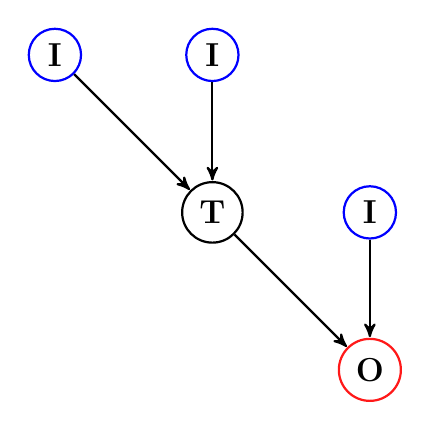
\begin{tikzpicture}[
	->,
	>=stealth',
	shorten >=.2pt,
	auto,
	node distance=2cm,
	thick,
	tmp node/.style={circle,draw,font=\large\bfseries},
	in node/.style={circle,draw=blue!100,font=\large\bfseries},
	out node/.style={circle,draw=red!90,font=\large\bfseries}
]

\node[in node] (1) {I};
\node[in node] (2) [right of=1] {I};
\node[tmp node] (3) [below of=2] {T};
\node[in node] (4) [right of=3] {I};
\node[out node] (5) [below of=4] {O};
%\node[main node] (1) {In};
%\node[main node] (2) [below left of=1] {2};
%\node[main node] (3) [below right of=2] {3};
%\node[main node] (4) [below right of=1] {4};

\path[every node/.style={font=\sffamily\small}]
(1) edge node [left] {} (3)
(2) edge node [left] {} (3)
(3) edge node [left] {} (5)
(4) edge node [left] {} (5)
;
%(1) edge node [left] {0.6} (4)
%%edge [bend right] node[left] {0.3} (2)
%edge [loop above] node {0.1} (1)
%(2) edge node [right] {0.4} (1)
%edge node {0.3} (4)
%edge [loop left] node {0.4} (2)
%edge [bend right] node[left] {0.1} (3)
%(3) edge node [right] {0.8} (2)
%edge [bend right] node[right] {0.2} (4)
%(4) edge node [left] {0.2} (3)
%edge [loop right] node {0.6} (4)
%edge [bend right] node[right] {0.2} (1);
\end{tikzpicture}
\caption{Graphical example of CDAG}
\label{fig:GraphCDAG}
\end{figure}

\section{VectorIR}
In order to approach the different architectures when generating instructions,
we need a generic vector representation of the vector instructions we want to
have in our program. For this purpose, MACVETH uses the VectorIR, that basically
wraps a set of nodes from the CDAG onto a common structure which represent a vector operation.

To wrap up: VectorIR is a generic way of representing vector operations for the different
architectures. Because of this, at this stage there is no fusing operations or
any other kind of target-specific optimizations. The concrete backend will be in
charge of doing this. For instance, AVX introduced the fuse add-multiplication
instructions often called FMAs, which as their name suggest fuse additions and
multiplication onto a single operation; however they are only available for FP
operations and, therefore, not for integers. It would be pointless to tackle
all these issues in this representation that is why this is done in the AVX
backend instead.

\section{SIMDBackEnd: \textit{the} backend}
In order to synthesize the vector operations gathered in the VectorIR, there
must exists a target-specific backend for each ISA. MACVETH disposes a general
interface called SIMDGenerator, which is connected to the front-end in order to
synthesize the SIMD or vectorized operations. This interface must be
implemented by each architecture and/or ISA in order to generate
target-specific code for each machine or system.

%\chapter{Vector API}
%In order to generate vector operations, the compiler basically generates a set 
%of wrap instructions substituting the original code. These wrap instructions 
%are defined 

%\chapter{$\mu$macro-bench}
%Architectures feature different 

\newpage
\chapter{Software Architecture}
MACVETH is built using LLVM framework in order to take advantage of the
sophisticated AST created when parsing files.

\bibliographystyle{unsrt}
\bibliography{sample}

\end{document}
%%%%%%%%%%%%%%%%%%%%%%%%%%%%%%%%%%%%%
